\documentclass[11pt]{article}

\usepackage[utf8]{inputenc}
\usepackage[T1]{fontenc}
\usepackage{lmodern}
\usepackage[margin=1in]{geometry}
\usepackage{amsmath}
\usepackage{graphicx}
\usepackage{booktabs}
\usepackage{caption}
\usepackage{enumitem}
\usepackage{placeins}
\usepackage{xcolor}
\usepackage[numbers,sort]{natbib}
\usepackage[colorlinks=true,linkcolor=blue!50!black,citecolor=blue!50!black,urlcolor=blue!50!black]{hyperref}

\graphicspath{{figures/}}
\captionsetup{font=small,labelfont=bf}
\setlist{itemsep=2pt,topsep=4pt}

\title{Buy the Better Guard: What a Fixed Oversight Budget Buys in Safety Moderation}
\author{Md.\ Zariful Huq\\
Software Engineer AI, Revora\\
\texttt{zarifhuq786@gmail.com}}
\date{}

\begin{document}

\maketitle

\begin{abstract}
Content moderation guard models are prone to errors, and practical deployments often address uncertain decisions by referring them to human reviewers. However, a fixed oversight budget can be allocated in several ways: using a larger guard model, spending additional compute to verify the guard's decisions, or increasing the amount of human review. These options compete for the same resources, yet, to the best of our knowledge, no previous work has systematically compared their costs and benefits. We investigate this trade-off using 26,958 predictions from three generative guard models across five moderation datasets. All experiments were conducted on a single machine under a protocol that was pre-registered before data collection began.

\textbf{Our results suggest that investing in a stronger guard model is generally the most effective strategy.} When results are pooled across all five datasets, the strongest individual guard, ranked using its own confidence scores without additional compute, produces the fewest incorrect decisions at human review rates of 1\%, 2\%, 5\%, and 50\%. A panel based on agreement among three guards performs better only at review rates between 10\% and 20\%, while requiring 2.5$\times$ more compute. The smallest guard does not outperform the alternatives at any review budget. Therefore, our pre-registered hypothesis that a low-cost guard combined with expensive verification would outperform a more expensive guard with no additional verification is not supported by the results. However, performance varies across individual datasets, indicating that the best strategy depends on the characteristics of the incoming traffic. On real user traffic (ToxicChat), the three-guard panel performs best at review rates between 2\% and 20\%.

The more important question is why these strategies have limited effectiveness. The main limitation is not computational capacity but error identification, specifically, the ability to determine which decisions are incorrect. An oracle routing strategy that selects whichever of two guards would produce the correct answer for each prompt could reduce errors by 26.3\% (95\% CI [23.5, 29.2]) while using half the compute required by the larger guard. However, the best available escalation signal fails to capture this potential improvement: its realized gain is $-0.0002$, which is statistically indistinguishable from zero (95\% CI [$-0.0017$, $+0.0012$]). This identification problem becomes more severe as input length increases. For 2.85\% of prompts, all three guards agree on the same answer, yet all three are incorrect, even though their confidence scores are high. The frequency of these failures increases by approximately ninefold between the shortest and longest fifths of prompts. Input length also affects the perturbation signal: the number of usable rewordings available for each prompt decreases as prompts become longer, with a rank correlation of $-1.0$ across datasets. Since benchmarks made up of short prompts contain relatively little variation in prompt length, they may fail to reveal both of these effects.

\medskip
\noindent Code and data: \url{https://github.com/zarif007/guard-uncertainty-routing}
\end{abstract}

\section{Introduction}

A guard model operates in front of a deployed language model and determines whether an incoming message should be allowed or blocked. However, guard models can make mistakes in both directions. They may block legitimate requests or allow harmful ones to pass through. To reduce these errors, operators often rely on human review, where uncertain decisions are referred to human reviewers. However, human review is a limited resource. In this study, we consider review rates of 1--20\% as a practical range for moderation teams, while treating 50\% as an upper reference point.

This limitation turns the operator's problem into a resource allocation challenge. Given a fixed oversight budget, an operator can invest in a larger and potentially more accurate guard model, allocate additional compute to verify the guard's decisions, or increase the amount of human review. Each option consumes resources that could otherwise be allocated to the alternatives. However, the relative benefits and costs of these choices remain unclear.

The closest related work is Safety-Flag~\cite{hu2026safetyflag}, which evaluates thirteen moderation models across seven datasets and shows that a model's own token-logprob confidence can be useful for ranking its incorrect decisions. The study considers the trade-off between missed harmful content and false alarms, but it does not account for computational costs or the resources required for human review. Furthermore, its reported risk measurements focus on 100\%, 80\%, and 50\% coverage, using datasets with an approximately equal distribution of harmful and benign samples. As a result, its reported results provide limited information about the 1--20\% review range that is particularly relevant to practical moderation deployments.

This paper focuses on that practical review range and examines how an operator should allocate a fixed oversight budget. Rather than proposing another general framework, our goal is to provide an empirical answer that practitioners can use when making deployment decisions. Our contributions are organized below in order of practical importance:

\begin{enumerate}
  \item \textbf{The allocation decision} (Section~\ref{sec:answer}). At the review rates commonly considered in this study, using a stronger guard model is generally more effective than spending additional compute on routing. The main exception is a review range of 10--20\%, where a panel of three guards performs better, although it requires 2.5$\times$ more compute. The smallest guard does not outperform the alternatives at any review rate.
  \item \textbf{A cost comparison of the available alternatives} (Sections~\ref{sec:method} and~\ref{sec:results}). We evaluate each combination of guard model, routing signal, and human review budget using two separate cost measures: computational requirements and human review. These costs are reported independently rather than converted into a common unit. The evaluation covers 26,958 predictions, with all experiments conducted on a single machine. To the best of our knowledge, previous work has not evaluated guard oversight using this form of cost comparison.
  \item \textbf{Why the alternatives underperform: the identification gap} (Section~\ref{sec:gap}). We distinguish between the improvement that routing could theoretically achieve and the improvement captured by currently available routing signals. We quantify this difference using bootstrap confidence intervals. Our results reveal a substantial gap between the potential benefit and the improvement achieved by practical signals, with the measured gain not being statistically distinguishable from zero.
  \item \textbf{Where identification breaks down: input length} (Section~\ref{sec:length}). We investigate how input length relates to two important failure patterns: cases where all guards produce the same incorrect decision and the declining effectiveness of the perturbation signal. Both patterns are associated with longer inputs, while benchmarks made up of short prompts contain relatively little variation in prompt length.
\end{enumerate}

\paragraph{Pre-registration.} The study hypotheses, decision thresholds, and evaluation gate structure were specified in a public repository before any predictions were generated. The protocol was then frozen after the first prediction was produced. Two important outcomes of this process are reflected in the paper, and we report both transparently. First, our principal hypothesis was not supported by the experimental results. Second, a mechanism proposed after examining the data was subsequently formalized, evaluated across eight panels, and rejected (Section~\ref{sec:rejected}).

\section{Related work}

\paragraph{Selective prediction for moderation.} Safety-Flag~\cite{hu2026safetyflag} evaluates the reliability and calibration of content moderation models across seven datasets and thirteen models. One of its key reliability metrics is the area under the risk-coverage curve (AURC)~\cite{elyaniv2010foundations,geifman2017selective}, which we also use as our primary ranking measure. The study shows that token-logprob confidence can effectively identify potentially incorrect predictions. It also finds that temperature scaling improves calibration without changing the relative ordering of predictions. We reproduce the first finding in our experiments (Section~\ref{sec:free}), while our results on logit margin provide a more detailed examination of the second finding.

Appendix D.1 of Safety-Flag also provides evidence against the effectiveness of behavioral signals. It reports that agreement among five sampled answers performs worse than token-logprob confidence across all six models evaluated. Our approach differs in that we introduce variation at the input level rather than the decoder level. This distinction is important because a guard evaluated greedily on a single label token has no sampling variance. Our findings in Section~\ref{sec:length} are consistent with the broader conclusion of Safety-Flag regarding the limitations of behavioral agreement as an uncertainty signal.

\paragraph{Uncertainty beyond confidence.} Semantic uncertainty~\cite{kuhn2023semantic} estimates a model's uncertainty by measuring how consistently its sampled outputs express the same meaning. We investigate a related idea by examining whether guard predictions remain consistent under meaning-preserving input variations, using these variations to identify potentially incorrect decisions. This approach changes the input rather than the generated output. However, a key concern is that prediction instability may simply provide information similar to a small confidence margin while requiring substantially more computation. Our gate S4 is designed to test this possibility directly. Previous work has also argued that entropy alone is insufficient for safe selective prediction~\cite{phillips2026entropy}, while abstention methods with formal guarantees have been developed for question-answering systems~\cite{dong2026abstention}. However, these approaches do not directly address the combined problem of moderation classification, limited human-review capacity, and computational cost.

\paragraph{Polarized guard scores.} A common concern when using guard verdict probabilities for ranking is that their scores may be concentrated near 0 or 1, leaving little variation to distinguish between predictions. If this were the case, confidence-based ranking would have limited practical value. Rather than assuming that such polarization occurs, we examine the score distributions of our own models. Our results show that 12--37\% of scores are pinned at the extremes, while the remaining scores retain sufficient variation to provide useful ranking information (Section~\ref{sec:free}).

\paragraph{Operating points and evaluation conditions.} Improving a safety detector's overall accuracy does not necessarily improve its performance at the operating points that matter in deployment. For example, reasoning can increase detection accuracy while reducing recall at the low false-positive rates required by practical systems~\cite{chegini2025razor}. Similarly, measured safety performance can vary depending on evaluation conditions, including answer formats and scoring rules~\cite{gringras2026scaffolding}. Other studies use a common decision threshold across models rather than selecting an appropriate threshold for each model individually~\cite{dacruz2026distillation}. In addition, classifier performance can change substantially under real distribution shifts~\cite{fomin2026benchmarks}. Our findings in Section~\ref{sec:choose} provide another example of why evaluation conditions and deployment operating points matter: a guard with a higher AUROC can still produce more errors once it is deployed at its default decision threshold.

\paragraph{What is not covered.} Despite these related developments, we find no prior study that jointly examines the computational and human-review costs of guard oversight. In particular, the existing literature does not tabulate performance across the 1--20\% human-review range, evaluate cross-model disagreement as a routing signal, or directly compare logit margin with probability-based confidence for this purpose. Our study addresses these gaps by evaluating these alternatives under a common experimental protocol and resource-constrained setting.

\section{Method}
\label{sec:method}

\subsection{Policies and the objective}

We define a \textbf{policy} as a combination of a guard model, a routing signal, and a human-review budget $b$. The routing signal assigns a score to every prompt, and the $b$ fraction of prompts with the lowest confidence scores is referred to a human reviewer. We assume that the reviewer correctly identifies and fixes every error presented to them. Our approach does not rely on predefined decision thresholds. Instead, it uses only the ranking induced by each routing signal. This allows different signals to be compared without requiring their scores to be calibrated onto a common scale.

Our primary evaluation objective is \textbf{residual risk}, defined as:
\[
\text{Residual risk} = \text{Errors made by the guard} - \text{Errors identified by the reviewer}.
\]
We report residual risk as a proportion of all evaluated prompts. We use this measure instead of accuracy or the number of errors caught because these alternatives can make weaker guard models appear more effective simply because they have more errors available to identify and correct. For example, a guard that makes 1,614 errors and has 1,128 of them caught by human review still allows more errors to pass through than a guard that makes 943 errors and has 561 corrected. Residual risk captures the number of errors that remain after human review and therefore provides a more direct measure of the outcome that matters in deployment.

\subsection{Two cost units, never mixed}

Computational resources and human-review time are fundamentally different types of costs. Converting them into a single measure would require assigning a monetary or operational value to each, and such an exchange rate may vary across organizations and change over time. Therefore, we keep these two costs separate throughout the study. Each policy is evaluated on a two-dimensional cost frontier, allowing practitioners to apply their own cost assumptions and determine which trade-off best fits their deployment requirements.

We measure compute as the median latency per decision, expressed in seconds, on the evaluation machine. For a panel consisting of multiple guards, every member processes every prompt. Its total computational cost is therefore calculated as the sum of the individual costs of all panel members. This cost represents the resources required to run the entire panel, regardless of which member's verdict is ultimately selected.

\subsection{Guards, data, and routing signals}

We evaluate three generative guard models, all running at fp16 precision through llama.cpp: Llama-Guard-3-8B~\cite{inan2023llamaguard}, Qwen3Guard-Gen-8B~\cite{zhao2025qwen3guard}, and Llama-Guard-3-1B~\cite{fedorov2024llamaguard1b}. Their overall performance and computational costs across the five datasets are summarized in Table~\ref{tab:guards}.

\begin{table}[ht]
\centering
\small
\caption{Performance of the three guard models and the combined three-guard panel across all five datasets. Compute represents the median latency in seconds per decision, measured on a single NVIDIA L40S.}
\label{tab:guards}
\begin{tabular}{lrrrr}
\toprule
guard & error rate & AUROC & flag rate & compute \\
\midrule
Llama-Guard-3-8B & 0.1049 & 0.9226 & 0.200 & 0.319 \\
Qwen3Guard-Gen-8B & 0.1157 & 0.9615 & 0.314 & 0.372 \\
Llama-Guard-3-1B & 0.1796 & 0.8704 & 0.283 & 0.102 \\
Three-guard panel & & & & 0.793 \\
\bottomrule
\end{tabular}
\end{table}

Our evaluation covers five moderation datasets containing 8,986 prompts after normalization, with a pooled harmful-content rate of 22.5\%. The datasets are ToxicChat~\cite{lin2023toxicchat} (4,972 prompts, 7.1\% harmful, representing real user traffic), WildGuardTest~\cite{han2024wildguard} (1,699 prompts), OpenAI Moderation~\cite{markov2023holistic} (1,665 prompts), XSTest~\cite{rottger2024xstest} (450 prompts, consisting of benign but borderline examples), and HarmBench~\cite{mazeika2024harmbench} (200 prompts, all harmful). Among these datasets, only ToxicChat has a harmful-content rate that reflects the low prevalence typically found in real user traffic. Consequently, the pooled dataset contains a higher proportion of harmful prompts than most practical moderation deployments. This distinction is important when interpreting the pooled results.

We evaluate four routing signals:
\begin{itemize}
  \item \textbf{Native confidence:} $|p_{\text{unsafe}} - 0.5|$, calculated after applying per-guard temperature scaling. This signal requires no additional inference and serves as our baseline.
  \item \textbf{Logit margin:} $|\text{margin}|$, which measures the absolute difference between the relevant output logits. Like native confidence, it is available without additional inference and therefore has no extra computational cost.
  \item \textbf{Three-guard agreement:} The proportion of guards that agree with the majority verdict. This signal requires all three guard models to process each prompt, resulting in three times the compute cost of a single-guard evaluation.
  \item \textbf{Perturbation instability:} The frequency with which a guard changes its verdict across six meaning-preserving rewordings of the original prompt. Evaluating this signal requires six additional evaluations, resulting in six times the compute cost.
\end{itemize}

The pre-registration also specifies a fifth routing signal based on the agreement of a single guard with itself across different quantization levels. However, this experiment was not conducted because the quantized models were never evaluated as part of the prediction set.

\paragraph{Environment.} All 26,958 predictions were generated on a single NVIDIA L40S. Each prediction record includes a hash identifying the computational environment in which it was generated. Our analysis pipeline uses these hashes to prevent latency comparisons between predictions produced under different environments. This ensures that the reported computational costs are based on a consistent hardware and software configuration. However, these measurements should be interpreted as machine-specific results rather than universal estimates of model latency.

\section{Pre-registered gates}

Each gate can fail. Before scoring any real data, every gate was validated on synthetic inputs with known expected outcomes in both directions (13 of 13 checks passed). The evaluation thresholds were fixed prior to testing: a 5\% relative reduction in residual risk for the allocation gate, and an AURC difference of 0.01 for signal comparisons. Table~\ref{tab:gates} summarizes these pre-registered gates and their final outcomes.

\begin{table}[ht]
\centering
\small
\caption{Pre-registered gates and their outcomes.}
\label{tab:gates}
\begin{tabular}{llp{6.2cm}}
\toprule
Gate & Question & Result \\
\midrule
A1 & At matched compute, does anything beat the default? & \texttt{CHEAPER\_GUARD\_WINS} (a different guard, not a different signal; Section~\ref{sec:choose}) \\
A2 & Does the winner change with budget? & \texttt{BUDGET\_DEPENDENT} \\
S1 & Is native confidence usable? & \texttt{NATIVE\_USABLE} (3 of 3 guards) \\
S2 & Does the margin beat the probability? & \texttt{NO\_DIFFERENCE} \\
S3 & Does any alternative beat native confidence? & \texttt{ALTERNATIVE\_BEATS\_NATIVE} (1 of 3 guards) \\
S4 & Is instability independent of the margin? & \texttt{INDEPENDENT}, narrowly, on 650 short prompts (Section~\ref{sec:length}) \\
S5 & Does guard \emph{kind} decide usability? & Not tested: no suitable encoder guard \\
\bottomrule
\end{tabular}
\end{table}

\section{Results}
\label{sec:results}

\subsection{The optimal strategy: deploy a stronger single guard}
\label{sec:answer}

\begin{table}[ht]
\centering
\small
\caption{The lowest-risk policy at each human-review rate, pooled over all five datasets.}
\label{tab:winners}
\begin{tabular}{rlrr}
\toprule
Review rate & Winning policy & Residual risk & Compute \\
\midrule
1\% & Llama-Guard-3-8B + own confidence & 0.0999 & 0.319 \\
2\% & Llama-Guard-3-8B + own confidence & 0.0963 & 0.319 \\
5\% & Llama-Guard-3-8B + own confidence & 0.0832 & 0.319 \\
10\% & Qwen3Guard-8B + 3-guard panel & 0.0634 & 0.793 \\
20\% & Qwen3Guard-8B + 3-guard panel & 0.0376 & 0.793 \\
50\% & Llama-Guard-3-8B + own confidence & 0.0112 & 0.319 \\
\bottomrule
\end{tabular}
\end{table}

Across most practical human-review rates (1\%, 2\%, and 5\%), as well as at a 50\% review baseline, the most effective policy is a single strong guard utilizing its inherent confidence score (Table~\ref{tab:winners}, Figure~\ref{fig:crossover}). This approach requires only a single forward pass per input and avoids additional infrastructure overhead.

Figure~\ref{fig:frontier} details the trade-off across all evaluated policies, mapping compute costs against residual risk. At review rates below 10\%, no setup costing more than Llama-Guard-3-8B running on its native confidence achieves a lower residual risk. At human-review rates of 10\% and 20\%, the multi-guard panel reaches the Pareto frontier, serving as the sole configuration where additional compute yields lower residual risk.

This 10--20\% review window is the single exception where a three-guard agreement panel outperforms the single guard, albeit at 2.5$\times$ the computational cost. Because this behavior does not scale monotonically with the review rate, Section~\ref{sec:rejected} tests one plausible explanation for this band and shows that the data do not support it.

Crucially, the smallest model (1B) never achieves the lowest risk at any review rate. These empirical results do not support our pre-registered hypothesis that combining a lightweight guard with selective, high-cost oversight would outperform a larger guard operating with zero-cost native confidence.

\begin{figure}[t]
\centering
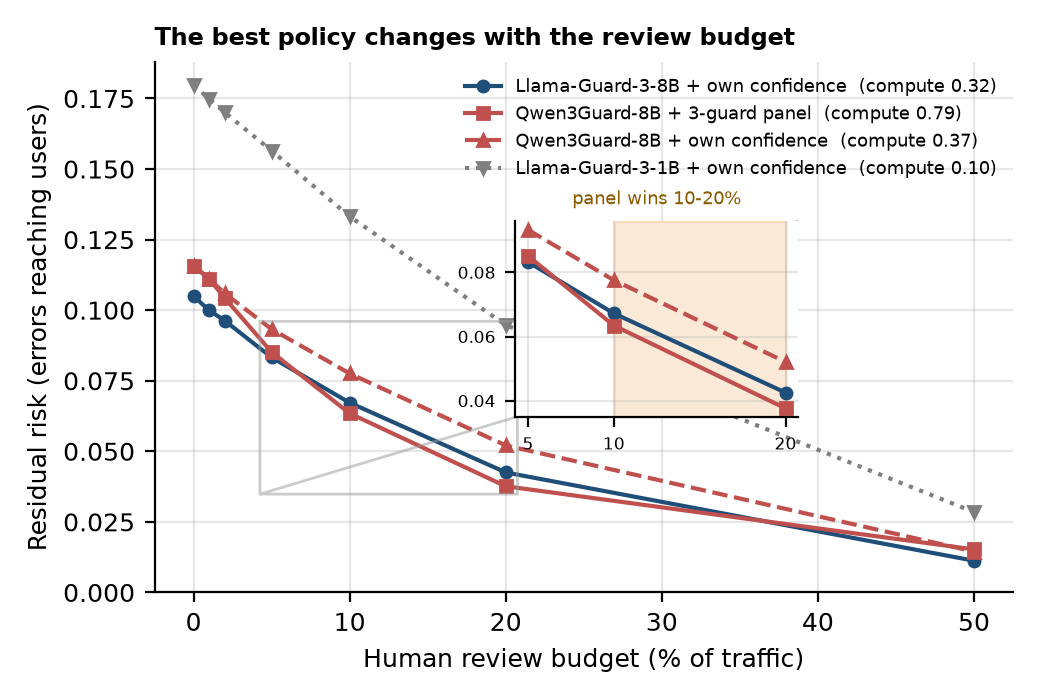
\includegraphics[width=0.8\linewidth]{figures/fig1_budget_crossover.png}
\caption{Residual risk across human-review rates for four routing policies. Llama-Guard-3-8B using native confidence achieves the lowest risk below a 10\% review rate and at 50\%; the three-guard panel outperforms it only within the 10--20\% review band, requiring 2.5$\times$ the compute. The inset highlights the crossover point. The 1B guard fails to win at any review rate.}
\label{fig:crossover}
\end{figure}

\begin{figure}[t]
\centering
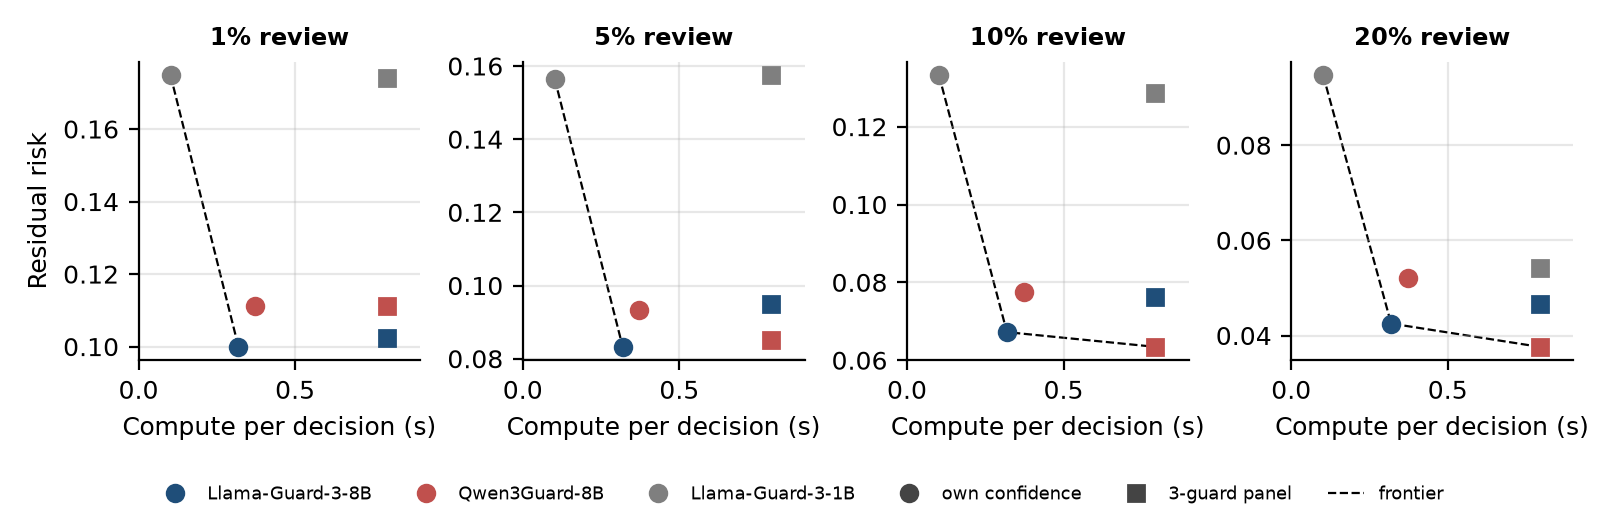
\includegraphics[width=\linewidth]{figures/fig2_oversight_frontier.png}
\caption{The oversight frontier across four human-review rates. Each point represents a policy plotted by inference latency (median seconds on a single NVIDIA L40S) against residual risk. Circles denote a guard using its native confidence score; squares represent a three-guard agreement panel (costing the sum of all three models). The dashed line marks the optimal frontier. While the 1B guard lies on the frontier due to low compute costs, it never achieves the lowest risk.}
\label{fig:frontier}
\end{figure}

\paragraph{Traffic composition dictates dataset-level performance.} While these primary results aggregate performance across five pre-registered datasets, individual dataset breakdowns in Appendix~\ref{app:per-dataset} reveal two important nuances. First, the optimal single guard varies by dataset: Qwen3Guard-Gen-8B achieves the lowest error on XSTest, HarmBench, and WildGuardTest. Llama-Guard-3-8B leads in the aggregated evaluation mainly because Qwen3Guard exhibits a high false-positive rate on OpenAI Moderation (0.279 error versus 0.130). Second, the panel wins more often within single datasets than in the pooled results, most clearly on ToxicChat, the only dataset reflecting realistic harm prevalence. There, the panel outperforms the best single guard at 2\%, 5\%, 10\%, and 20\% review rates, reducing residual risk by 2--23\% relative. Overall, across all 30 evaluated combinations of datasets and review rates, a single guard using native confidence wins in 22 settings, whereas the panel wins in 8. The smallest guard never achieves the lowest risk outright in any setting.

The remainder of this section analyzes why alternative routing strategies usually fail to beat native confidence, focusing on insights that are likely to apply beyond the specific models evaluated here.

\subsection{Native confidence signals are effective and hard to augment for free}
\label{sec:free}

All three evaluated guards provide useful native confidence estimates, demonstrating deferral efficiencies between 0.667 and 0.745 and score tie fractions below 0.003 (Figure~\ref{fig:riskcov}). This confirms the findings of Safety-Flag~\cite{hu2026safetyflag} for Llama-Guard-3-8B and extends those results to two additional guard models. Furthermore, it clarifies why simple single-guard routing works so well: the default confidence metric is already surprisingly effective.

\begin{figure}[t]
\centering
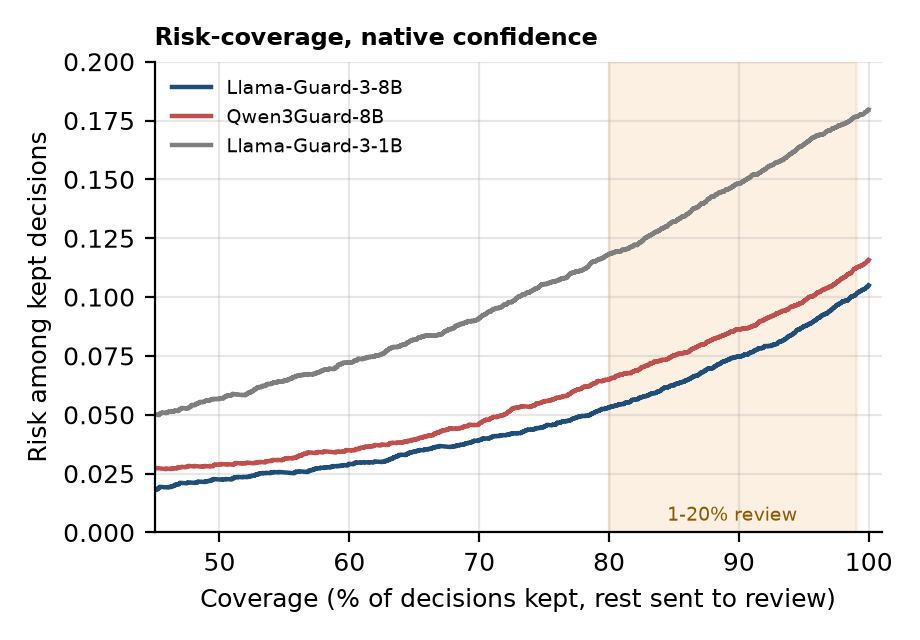
\includegraphics[width=0.7\linewidth]{figures/fig3_risk_coverage.png}
\caption{Risk-coverage curves for native confidence across all three guards, pooled over five datasets. The error rate among the decisions a guard keeps decreases as more uncertain cases are routed to human review. The shaded band marks the primary 1--20\% review target of this study.}
\label{fig:riskcov}
\end{figure}

Attempting to improve this zero-cost signal using raw logit margins provides no additional benefit. We initially hypothesized that logit margins would retain fine-grained ranking information that is lost when the sigmoid function saturates near extreme values. In practice, ranking by raw logit margin produces identical results to ranking by output probability: the AUROC values are identical across all three guards, and the resulting AURC values differ by less than $1.8 \times 10^{-8}$. This saturation never occurred in our data. The median absolute margin spans from 4.0 to 5.8, well below the threshold of approximately 37 where floating-point operations round to 1.0, with only 12--37\% of output scores resting at extreme values.

Consequently, common assumptions about guard probability outputs being uninformative or degenerate do not hold for these models. Uncertainty behaviors should be measured empirically on target architectures rather than assumed.

\subsection{Multi-guard panels offer narrow benefits restricted to weaker models}

When evaluating a three-guard voting panel, consensus decisions yield only discrete outcome counts. The tie fraction across all prompts and datasets reaches 1.0; the panel effectively splits traffic into a flagged group (where models disagree) and an unflagged group, but provides no fine-grained ranking within either category. Because of this coarse ranking, panel routing improves performance only within a narrow range of human-review rates.

Across the benchmark traffic, the disagreement group covers 23.8\% of prompts (2,141 samples) and captures 72.9--84.1\% of all errors made by individual guards. However, as shown in Table~\ref{tab:agree} and Figure~\ref{fig:forest}, the performance gains from panel voting are not uniform across models.

\begin{table}[ht]
\centering
\small
\caption{Change in AURC when adopting three-guard panel agreement compared to native confidence. Negative values indicate performance improvements; p-values reflect Holm adjustment~\cite{holm1979simple}.}
\label{tab:agree}
\begin{tabular}{lrcr}
\toprule
Guard & Change in AURC & 95\% CI & Holm $p$ \\
\midrule
Llama-Guard-3-1B & $-0.0142$ & [$-0.0201$, $-0.0085$] & 0.000 \\
Llama-Guard-3-8B & $+0.0158$ & [$+0.0101$, $+0.0204$] & 1.000 \\
Qwen3Guard-8B & $+0.0092$ & [$-0.0011$, $+0.0103$] & 1.000 \\
\bottomrule
\end{tabular}
\end{table}

While panel agreement yields a statistically significant improvement for the smaller 1B model, the estimated effect points in the wrong direction for both 8B guards, and neither of those differences is significant after correction. A stronger guard model does not benefit from consulting weaker models in an agreement panel. This highlights a critical limitation, as ensemble disagreement is often assumed to be universally helpful without considering individual model capacity.

\begin{figure}[t]
\centering
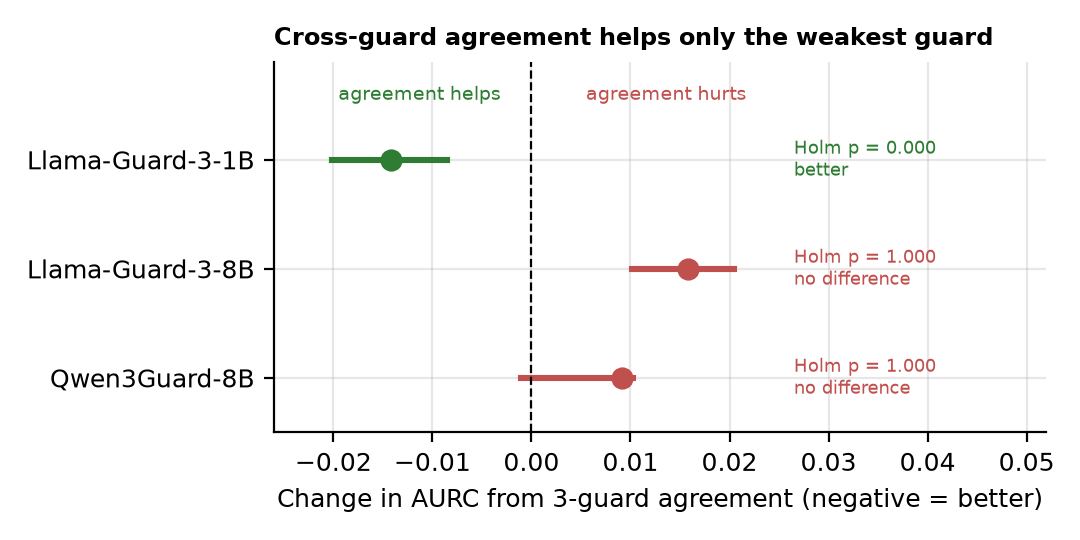
\includegraphics[width=0.75\linewidth]{figures/fig4_agreement_forest.png}
\caption{AURC differences resulting from three-guard agreement panels relative to native confidence, alongside 95\% bootstrap confidence intervals and Holm-corrected p-values. Only the 1B model shows a measurable improvement; for both 8B models the estimate points the wrong way, and neither difference survives correction.}
\label{fig:forest}
\end{figure}

\subsection{Quantifying the identification gap}
\label{sec:gap}

In the standard single-guard policies, one model evaluates every incoming prompt. To test whether dynamic allocation could improve efficiency, we evaluated a cascading policy: the 1B guard inspects all inputs, and its least confident 60\% of prompts are escalated to the 8B guard. This cascade is calculated directly from stored model predictions without requiring extra inference passes (Table~\ref{tab:cascade}). For comparison, an oracle baseline escalates only the specific prompts that the 1B model classifies incorrectly.

\begin{table}[ht]
\centering
\small
\caption{Evaluation of cascading setups between the 1B and 8B guards. Confidence intervals represent 95\% bootstrap estimates over 2,000 prompt resamples.}
\label{tab:cascade}
\begin{tabular}{lrcr}
\toprule
Policy & Error rate & 95\% CI & Compute \\
\midrule
8B alone & 0.1049 & [0.0985, 0.1113] & 0.319 \\
Cascade (escalating on 1B confidence) & 0.1052 & [0.0988, 0.1118] & 0.294 \\
Cascade (oracle escalation) & 0.0773 & [0.0717, 0.0830] & 0.159 \\
\bottomrule
\end{tabular}
\end{table}

Bootstrapping across prompts with 2,000 resamples yields two main findings:
\begin{itemize}
  \item \textbf{Realized gain} (8B alone minus practical cascade): $-0.0002$ (95\% CI: [$-0.0017$, $+0.0012$]), which spans zero and indicates no statistical difference.
  \item \textbf{Theoretical available gain} (8B alone minus oracle cascade): $+0.0276$ (95\% CI: [$+0.0243$, $+0.0310$]), which sits well above zero.
\end{itemize}

Because the 1B and 8B models make errors on different subsets of prompts, a perfect escalation mechanism could reduce overall error by 26.3\% (95\% CI: [23.5\%, 29.2\%]) while using only half the 8B model's compute budget (Figure~\ref{fig:gap}). However, existing confidence signals fail to capture this potential improvement.

Thus, deploying a larger single guard remains preferable to confidence-based routing not because dynamic allocation lacks theoretical value, but because current uncertainty signals cannot reliably trigger escalation when needed.

\begin{figure}[t]
\centering
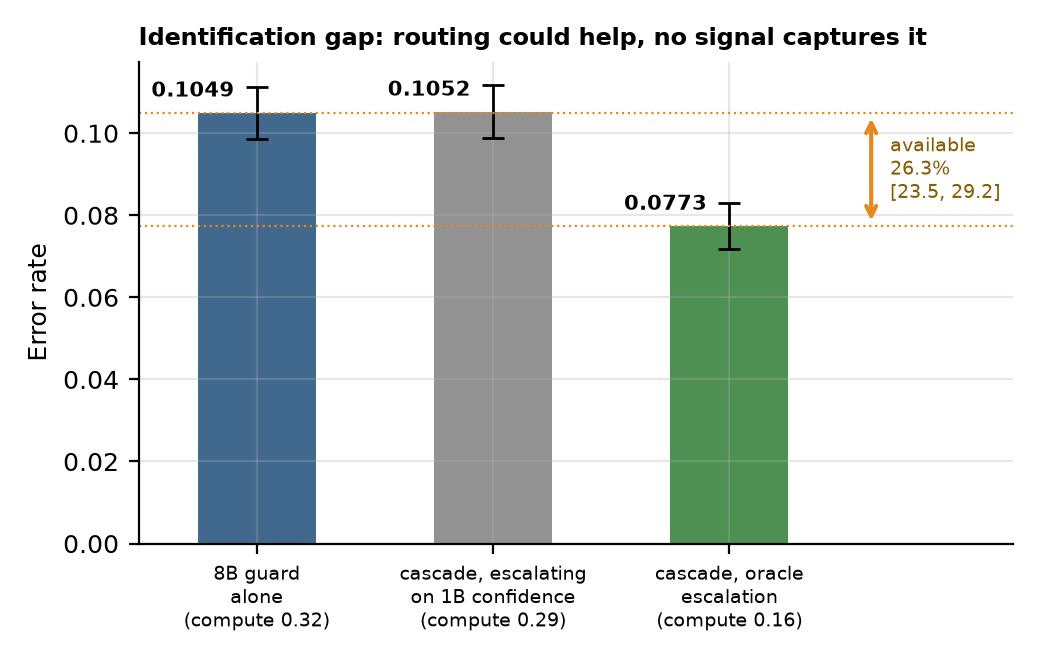
\includegraphics[width=0.75\linewidth]{figures/fig5_identification_gap.png}
\caption{The identification gap across routing strategies. Error bars represent 95\% bootstrap confidence intervals. Escalating based on 1B model confidence performs identically to using the 8B guard alone. An oracle escalation mechanism reduces error by 26.3\% at half the computational cost. The gap between these lines highlights uncaptured routing potential.}
\label{fig:gap}
\end{figure}

\subsection{Failures of identification: input length dynamics}
\label{sec:length}

Across the dataset suite, 2.85\% of prompts (256 samples) resulted in unanimous agreement across all three guards on an incorrect verdict: 167 benign prompts were falsely flagged, and 89 harmful prompts were incorrectly allowed through. Three structural factors explain why confidence-guided review policies fail to catch these unanimous errors.

\paragraph{Unanimous errors exhibit high overconfidence.} The median distance from the decision threshold, $|p - 0.5|$, ranges between 0.459 and 0.480 for unanimous errors, compared to 0.493 to 0.499 for unanimous correct predictions. Because guards are confident in their mistaken classifications, confidence-based ranking cannot flag these samples for human review.

\paragraph{Unanimous failure rates are concentrated in long-form datasets.} These failure cases do not occur uniformly across benchmark datasets. HarmBench contains no instances of unanimous failures, whereas the two long-form datasets show much higher unanimous-failure rates (Table~\ref{tab:unanimous}).

\begin{table}[ht]
\centering
\small
\caption{Frequency of unanimous guard errors broken down by dataset.}
\label{tab:unanimous}
\begin{tabular}{lrrr}
\toprule
Dataset & Total $n$ & Unanimous errors & Failure rate \\
\midrule
WildGuardTest & 1,699 & 87 & 5.12\% \\
OpenAI Moderation & 1,665 & 82 & 4.92\% \\
XSTest & 450 & 11 & 2.44\% \\
ToxicChat & 4,972 & 76 & 1.53\% \\
HarmBench & 200 & 0 & 0.00\% \\
\bottomrule
\end{tabular}
\end{table}

\paragraph{Prompt length correlates with error concentration.} Within individual datasets, inputs that produce unanimous errors tend to be longer than the rest of the same dataset: 967 vs.\ 363 characters in OpenAI Moderation, 548 vs.\ 236 in WildGuardTest, 83 vs.\ 59 in ToxicChat, and 45 vs.\ 42 in XSTest, where the difference is small. Grouping prompts into length quintiles reveals an overall increase in unanimous failure rates, rising from 0.65\% for the shortest inputs (median 30 characters) to 6.12\% for the longest (median 869 characters), representing a roughly ninefold increase, although the fourth quintile (2.28\%) dips below the third (3.07\%) (Figure~\ref{fig:length}a).

Input length also affects semantic perturbation testing. Meaning-preserving surface edits (such as adding greetings or expanding contractions) were used to test prediction stability. However, a pre-inference quality filter rejected three of the five datasets because the generated perturbations failed to achieve sufficient variation from the original text (Table~\ref{tab:variants}).

\begin{table}[ht]
\centering
\small
\caption{Usable text rewordings generated per prompt across datasets. Datasets averaging fewer than 4 valid variants were excluded prior to inference.}
\label{tab:variants}
\begin{tabular}{lrr}
\toprule
Dataset & Mean prompt length (chars) & Usable variants (out of 6) \\
\midrule
XSTest & 44 & 5.0 \\
HarmBench & 89 & 4.4 \\
ToxicChat & 167 & 3.5 (excluded) \\
WildGuardTest & 480 & 2.4 (excluded) \\
OpenAI Moderation & 645 & 2.0 (excluded) \\
\bottomrule
\end{tabular}
\end{table}

We observe a strong inverse rank correlation ($-1.0$) between average prompt length and usable rewordings (Figure~\ref{fig:length}b). This is driven by simple arithmetic: localized text modifications represent a smaller overall proportion of longer inputs, minimizing their impact on model processing.

For the two datasets that passed validation (650 short prompts using Llama-Guard-3-8B), prediction instability provides information that is distinct from the logit margin, narrowly satisfying Gate S4 with a correlation of 0.49 against the 0.5 threshold. However, prediction instability still performs worse than native confidence at prioritizing errors for review. On XSTest, instability achieves an AURC of 0.0295 compared to 0.0157 for native confidence, identifying 10 errors at a 5\% review rate versus 12 identified by native confidence. On HarmBench, instability performs worse than random selection, missing all 5 errors at a 5\% review rate where native confidence identifies 3. Crucially, generating these perturbation metrics requires six times the compute budget of standard inference.

\begin{figure}[t]
\centering
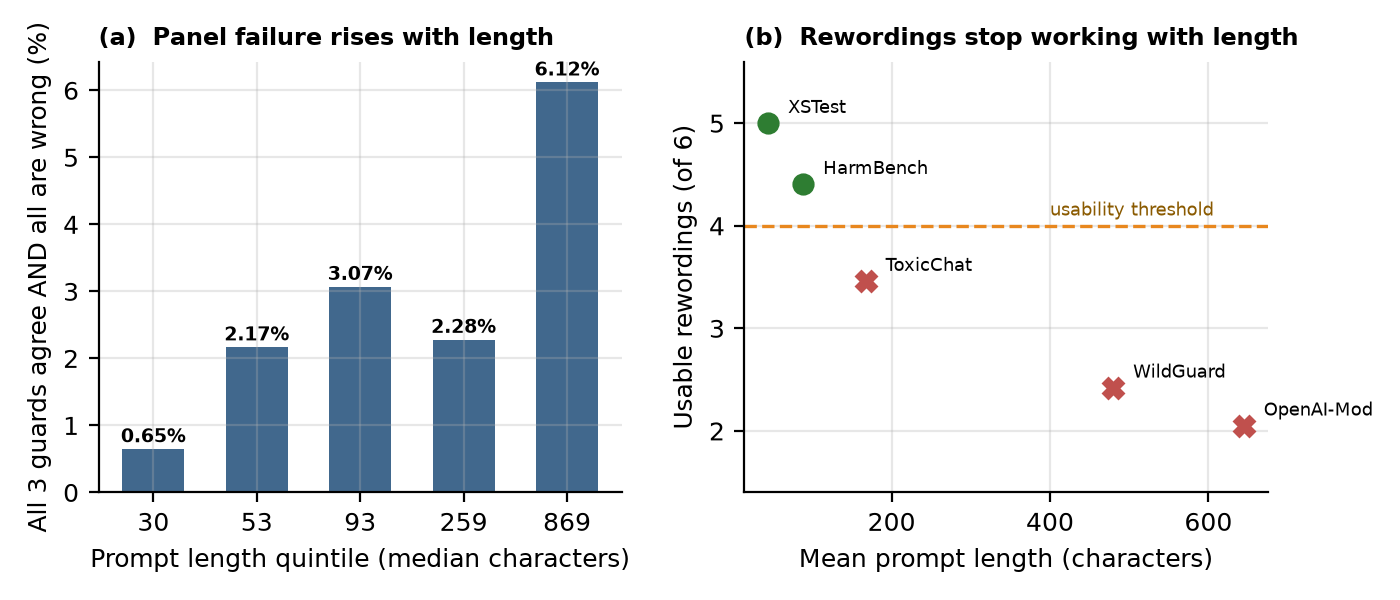
\includegraphics[width=\linewidth]{figures/fig6_length_axis.png}
\caption{Input length affects safety oversight performance. Subfigure (a) illustrates the rate of unanimous guard errors across prompt length quintiles, rising from 0.65\% for short inputs to 6.12\% for long inputs. Subfigure (b) shows the inverse relationship between prompt length and the number of usable text rewordings across datasets.}
\label{fig:length}
\end{figure}

These findings indicate that guard oversight mechanisms encounter compounding vulnerabilities on long inputs. Uncertainty signals fail to route long-form inputs effectively, precisely where consensus voting and agreement panels are most likely to make shared errors. Benchmarks composed primarily of short prompts mask this behavior by controlling for input length.

\subsection{Evaluation metrics vs.\ deployment performance}
\label{sec:choose}

While the optimal overall strategy is to deploy a stronger individual guard, selecting which guard to deploy requires careful metric alignment.

Gate A1 indicates that, at matched compute levels, one configuration outperforms the default baseline by 10.7\%. In this benchmark, the default baseline is Qwen3Guard-Gen-8B paired with its native confidence score, while the higher-performing option is Llama-Guard-3-8B utilizing its native confidence at 0.86$\times$ the compute. Because both configurations use the same underlying signal type, this performance gap reflects differences between the guard models themselves rather than alternative routing mechanisms.

Qwen3Guard achieves the higher AUROC score of the two models (0.9615 versus 0.9226), yet yields a higher deployment error rate (0.1157 versus 0.1049). This discrepancy occurs because Qwen3Guard's default decision boundary over-flags traffic, marking 31.4\% of inputs as unsafe despite an underlying dataset harm rate of 22.5\% (Figure~\ref{fig:auroc}). Evaluating models strictly by AUROC favors Qwen3Guard, whereas evaluating by deployed residual risk favors Llama-Guard-3-8B. Standard model evaluations mostly report AUROC, which can obscure these operational trade-offs.

Furthermore, relative model rankings remain dependent on traffic distribution. As detailed in Appendix~\ref{app:per-dataset}, Qwen3Guard achieves lower error on three of the five individual datasets, whereas Llama-Guard-3-8B performs better on one dataset, and both models yield similar results on ToxicChat. Consequently, identifying the most effective guard model depends on both model characteristics and deployment traffic patterns, requiring evaluation on inputs that accurately reflect expected operational conditions.

\begin{figure}[t]
\centering
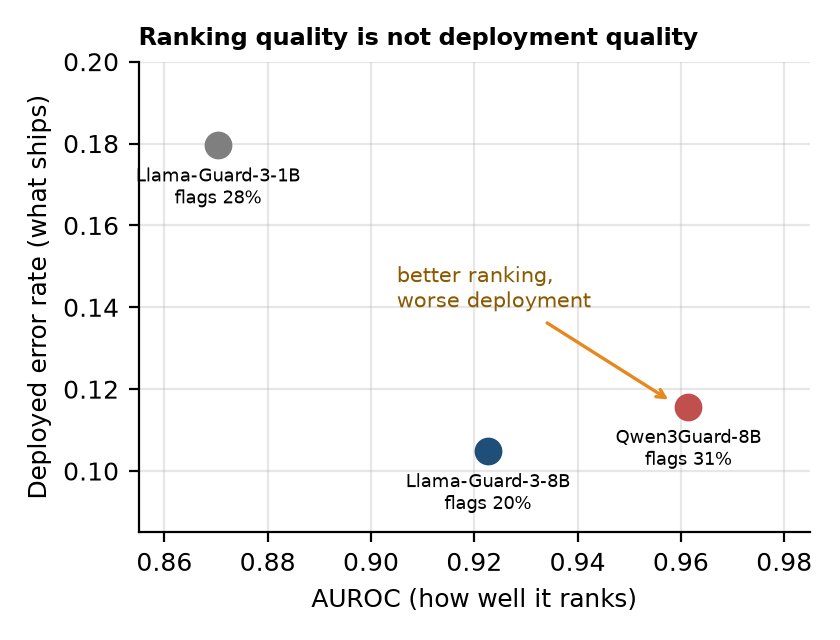
\includegraphics[width=0.6\linewidth]{figures/fig7_auroc_vs_error.png}
\caption{Comparison of ranking capability (AUROC) against deployment error rate. Qwen3Guard-Gen-8B achieves the highest AUROC but results in higher deployment error due to over-flagging 31.4\% of inputs against a 22.5\% ground-truth harm rate.}
\label{fig:auroc}
\end{figure}

\section{Discussion}

\paragraph{Deployment recommendations.} For human-review rates below 10\%, system designers should deploy the strongest available single guard model paired with its native confidence metric, spending no compute budget on explicit routing. Within the 10--20\% review window, a three-guard agreement panel justifies its 2.5$\times$ computational cost. Beyond a 20\% review rate, deployment policy should revert to the single strong guard. Crucially, the preferred guard model must be selected based on deployed residual risk on expected production traffic rather than AUROC scores (Section~\ref{sec:choose}). Because these guidelines stem from aggregated dataset benchmarks, operational trade-offs can vary; on distributions such as ToxicChat, panel routing yields benefits at review rates as low as 2\% (Appendix~\ref{app:per-dataset}). Consequently, deployment crossover thresholds should be measured on target traffic rather than assumed.

\paragraph{Underlying performance factors.} We evaluated five distinct strategies for reducing residual risk, and each encountered a clear performance ceiling (Table~\ref{tab:routes}).

\begin{table}[ht]
\centering
\small
\caption{Evaluated oversight strategies and their key performance constraints.}
\label{tab:routes}
\begin{tabular}{lp{8.5cm}}
\toprule
Strategy & Constraint \\
\midrule
Logit margin & Ranks predictions identically to raw output probability \\
Perturbation instability & Unmeasurable on realistic prompt lengths; underperforms native confidence on short prompts \\
Cross-model disagreement & Provides only two distinct values; yields risk reductions only within a 10--20\% review window \\
Cascaded escalation & Fails to capture any of the 0.0276 theoretical risk reduction \\
Multi-guard panels & Unanimous, overconfident errors persist across 2.85\% of evaluated inputs \\
\bottomrule
\end{tabular}
\end{table}

These boundaries are not driven by hardware limitations, as inference compute was allocated freely throughout testing. Instead, each restriction reflects a failure of current uncertainty signals to identify incorrect guard decisions. As quantified in Section~\ref{sec:gap}, existing signals fail to capture a 26.3\% potential error reduction.

\paragraph{Directions for future research.} Because both signal collapse and unanimous guard errors are associated with prompt length, evaluations restricted to short prompts understate both failure modes. Developing robust oversight signals requires perturbations that scale effectively with longer inputs. While neural paraphrasers offer semantic flexibility, they introduce a critical evaluation confound: automated rewording can inadvertently sanitize harmful prompts, making verdict flips difficult to interpret. Resolving this evaluation challenge represents a more impactful path forward than searching for additional zero-shot heuristics.

\section{Analysis of a rejected mechanism}
\label{sec:rejected}

A plausible hypothesis for the 10--20\% review window identified in Section~\ref{sec:answer} is that panel agreement benefits diminish once human-review capacity exceeds the proportion of traffic flagged for disagreement. This hypothesis predicts that the advantage of panel routing ends precisely at its disagreement flag rate. To evaluate this hypothesis, we computed pair and triple panel combinations across an empirical grid spanning 1--50\% review rates, breaking ties randomly across 20 random seeds.

The empirical data contradicts this prediction. Across the eight panel configurations that outperform native confidence at some review rate, the Spearman correlation between panel flag rate and the upper bound of that winning range is only 0.435. Furthermore, the winning range extends past the panel flag rate across all eight configurations, exceeding it by an average of 0.155. Thus, the flag rate marks the point where panel routing stops gaining relative advantage, rather than where it ceases to lead over single-guard policies. We report this negative result to clarify the operational behavior of voting panels.

\section{Limitations}

\begin{enumerate}
  \item \textbf{Hardware configuration.} Compute latency measurements were collected strictly on a single NVIDIA L40S GPU. On this hardware, Gate A1 finds that Llama-Guard-3-8B on its own confidence beats the default policy at lower compute, but different hardware architectures or batching setups may shift relative compute rankings and change which policy counts as the default.
  \item \textbf{Evaluated signal diversity.} Panel agreement served as the primary alternative routing signal with complete benchmark coverage. Signal S2 yielded no statistical difference, S4 was restricted to 650 short prompts on a single guard, and S5 could not be evaluated because no suitable encoder guard was available.
  \item \textbf{Absence of encoder guards.} The candidate encoder model achieved an AUROC of only 0.599 relative to our evaluation targets (attributable to detecting general toxicity rather than harmful requests) and was excluded prior to final scoring. Consequently, Gate S5 remains unevaluated.
  \item \textbf{Dataset harm prevalence.} The aggregated evaluation benchmark exhibits a 22.5\% harmful prompt rate. Only ToxicChat (7.1\%) reflects the lower prevalence rates typical of production environments. As noted in Appendix~\ref{app:per-dataset}, multi-guard panels outperform single guards across a broader range of review budgets on ToxicChat than in the aggregated benchmark.
  \item \textbf{Idealized human oversight.} The evaluation framework assumes perfect human review precision, treating ground-truth dataset labels as flawless oracle corrections.
  \item \textbf{Exploratory post-hoc analyses.} The empirical findings in Sections~\ref{sec:gap}, \ref{sec:length}, and~\ref{sec:rejected} are exploratory and were derived after inspecting the pre-registered primary outcomes. The oracle cascade bound in Section~\ref{sec:gap} applies specifically to the evaluated 1B and 8B guard pair.
  \item \textbf{Correlational length effects.} Although length dependencies persist within individual datasets, input length may correlate with underlying topic complexity or prompt structure.
  \item \textbf{Scope of perturbation testing.} Perturbation analysis was restricted to lightweight surface edits. Paraphrase models were excluded to prevent semantic sanitization, meaning Section~\ref{sec:length} bounds surface-level edits rather than behavioral perturbations in general.
\end{enumerate}

\section{Conclusion}

When deploying content moderation guards under fixed human-review capacity, organizations should \textbf{invest in stronger standalone guard models rather than complex routing mechanisms}. Across practical deployment review rates, alternative routing strategies fail to outperform a strong single model using native confidence outside a narrow 10--20\% review window, while lightweight models fail to achieve optimal risk reduction at any review budget. Because model selection and panel efficacy depend on input distributions, optimal configurations must be validated on production-representative traffic.

While these empirical findings diverge from our initial pre-registered hypothesis, they provide a concrete measurement of the trade-offs governing safety oversight.

The underlying cause of this performance ceiling is directly measurable: perfect routing between existing guard pairs could cut classification error by a quarter while halving compute costs, yet current uncertainty signals fail to capture this opportunity. Safety oversight encounters its greatest failures on long-form inputs, where multi-guard panels make confident, unanimous errors and standard routing signals lose discriminative power.

\section*{Ethics statement}

This study evaluates content moderation classifiers on publicly available benchmarks containing harmful and offensive language. The evaluation methodology generates no original harmful content; all perturbation tests rely strictly on surface edits of existing benchmark prompts. We release model predictions rather than new prompt instances. For datasets subject to non-commercial licenses or restricted access, released artifact files omit raw prompt strings, allowing researchers to rejoin text fields from primary source repositories.

\section*{Reproducibility}

All project assets, including the pre-registration protocol, analysis scripts, 26,958 model predictions, and data processing pipelines required to reproduce all figures and tables, are publicly available at \url{https://github.com/zarif007/guard-uncertainty-routing}. Pre-registered evaluation gates were validated against synthetic ground-truth test cases (13 of 13 checks passed). Claims are licensed by an automatically generated evidence table rather than chosen by hand, and claims that table does not license are not made here. All figures and tables can be recomputed from released predictions without GPU hardware requirements.

\bibliographystyle{unsrtnat}
\bibliography{references}

\clearpage
\appendix
\FloatBarrier

\section{Results per dataset}
\label{app:per-dataset}

These tables split the pooled results by dataset. They are exploratory: the pre-registered analysis is pooled. Review budgets apply within each dataset.

\begin{table}[ht]
\centering
\small
\caption{Error rate of each guard, by dataset. The lowest error in each row is in bold.}
\label{tab:per-dataset-error}
\begin{tabular}{lrrrrr}
\toprule
dataset & $n$ & harmful & Llama-Guard-3-8B & Qwen3Guard-8B & Llama-Guard-3-1B \\
\midrule
ToxicChat & 4,972 & 7.1\% & \textbf{0.077} & 0.078 & 0.162 \\
WildGuardTest & 1,699 & 44.4\% & 0.172 & \textbf{0.089} & 0.201 \\
OpenAI Moderation & 1,665 & 30.9\% & \textbf{0.130} & 0.279 & 0.234 \\
XSTest & 450 & 44.4\% & 0.096 & \textbf{0.082} & 0.151 \\
HarmBench & 200 & 100.0\% & 0.025 & \textbf{0.000} & 0.050 \\
\bottomrule
\end{tabular}
\end{table}

Table~\ref{tab:per-dataset-winners} gives the lowest-risk policy for each dataset and review budget. ``Own'' is a guard on its own confidence; ``panel'' is that guard deciding, with three-guard agreement choosing what to review. Ties go to the cheaper policy, which is why the 1B appears on HarmBench at 50\% review, where every policy reaches zero. Rows where the panel wins are in bold.

\begin{table}[ht]
\centering
\caption{Lowest-risk policy by dataset and review budget, with the best single-guard policy for comparison.}
\label{tab:per-dataset-winners}
\resizebox{\linewidth}{!}{%
\begin{tabular}{lrlrlr}
\toprule
dataset & budget & best policy & residual & best single guard & residual \\
\midrule
ToxicChat & 1\% & Llama-Guard-3-8B + own & 0.0720 & Llama-Guard-3-8B + own & 0.0720 \\
\textbf{ToxicChat} & \textbf{2\%} & \textbf{Llama-Guard-3-8B + panel} & \textbf{0.0664} & Llama-Guard-3-8B + own & 0.0680 \\
\textbf{ToxicChat} & \textbf{5\%} & \textbf{Llama-Guard-3-8B + panel} & \textbf{0.0533} & Llama-Guard-3-8B + own & 0.0563 \\
\textbf{ToxicChat} & \textbf{10\%} & \textbf{Qwen3Guard-8B + panel} & \textbf{0.0396} & Qwen3Guard-8B + own & 0.0426 \\
\textbf{ToxicChat} & \textbf{20\%} & \textbf{Llama-Guard-3-8B + panel} & \textbf{0.0171} & Qwen3Guard-8B + own & 0.0223 \\
ToxicChat & 50\% & Qwen3Guard-8B + own & 0.0040 & Qwen3Guard-8B + own & 0.0040 \\
\midrule
WildGuardTest & 1\% & Qwen3Guard-8B + own & 0.0836 & Qwen3Guard-8B + own & 0.0836 \\
WildGuardTest & 2\% & Qwen3Guard-8B + own & 0.0806 & Qwen3Guard-8B + own & 0.0806 \\
WildGuardTest & 5\% & Qwen3Guard-8B + own & 0.0689 & Qwen3Guard-8B + own & 0.0689 \\
WildGuardTest & 10\% & Qwen3Guard-8B + own & 0.0577 & Qwen3Guard-8B + own & 0.0577 \\
WildGuardTest & 20\% & Qwen3Guard-8B + own & 0.0365 & Qwen3Guard-8B + own & 0.0365 \\
WildGuardTest & 50\% & Qwen3Guard-8B + own & 0.0129 & Qwen3Guard-8B + own & 0.0129 \\
\midrule
\textbf{OpenAI Moderation} & \textbf{1\%} & \textbf{Llama-Guard-3-8B + panel} & \textbf{0.1261} & Llama-Guard-3-8B + own & 0.1267 \\
OpenAI Moderation & 2\% & Llama-Guard-3-8B + own & 0.1213 & Llama-Guard-3-8B + own & 0.1213 \\
OpenAI Moderation & 5\% & Llama-Guard-3-8B + own & 0.1081 & Llama-Guard-3-8B + own & 0.1081 \\
OpenAI Moderation & 10\% & Llama-Guard-3-8B + own & 0.0853 & Llama-Guard-3-8B + own & 0.0853 \\
OpenAI Moderation & 20\% & Llama-Guard-3-8B + own & 0.0649 & Llama-Guard-3-8B + own & 0.0649 \\
OpenAI Moderation & 50\% & Llama-Guard-3-8B + own & 0.0192 & Llama-Guard-3-8B + own & 0.0192 \\
\midrule
\textbf{XSTest} & \textbf{1\%} & \textbf{Qwen3Guard-8B + panel} & \textbf{0.0756} & Qwen3Guard-8B + own & 0.0800 \\
XSTest & 2\% & Qwen3Guard-8B + own & 0.0711 & Qwen3Guard-8B + own & 0.0711 \\
\textbf{XSTest} & \textbf{5\%} & \textbf{Qwen3Guard-8B + panel} & \textbf{0.0578} & Qwen3Guard-8B + own & 0.0622 \\
\textbf{XSTest} & \textbf{10\%} & \textbf{Qwen3Guard-8B + panel} & \textbf{0.0378} & Llama-Guard-3-8B + own & 0.0422 \\
XSTest & 20\% & Llama-Guard-3-8B + own & 0.0244 & Llama-Guard-3-8B + own & 0.0244 \\
XSTest & 50\% & Qwen3Guard-8B + own & 0.0000 & Qwen3Guard-8B + own & 0.0000 \\
\midrule
HarmBench & 1\% & Qwen3Guard-8B + own & 0.0000 & Qwen3Guard-8B + own & 0.0000 \\
HarmBench & 2\% & Qwen3Guard-8B + own & 0.0000 & Qwen3Guard-8B + own & 0.0000 \\
HarmBench & 5\% & Qwen3Guard-8B + own & 0.0000 & Qwen3Guard-8B + own & 0.0000 \\
HarmBench & 10\% & Qwen3Guard-8B + own & 0.0000 & Qwen3Guard-8B + own & 0.0000 \\
HarmBench & 20\% & Llama-Guard-3-8B + own & 0.0000 & Llama-Guard-3-8B + own & 0.0000 \\
HarmBench & 50\% & Llama-Guard-3-1B + own & 0.0000 & Llama-Guard-3-1B + own & 0.0000 \\
\bottomrule
\end{tabular}%
}
\end{table}

\end{document}
